\chapter{\babTiga}

%---------------------------------------------------------
\section{Eksperimen Awalan}
%---------------------------------------------------------
Sebelum penulis membuat proposal, penulis telah melakukan beberapa eksperimen kecil untuk mengetahui seberapa memungkinkannya ABS digunakan untuk pengembangan aplikasi berbasis web. Penelitian kecil yang telah dilakukan antara lain adalah:

\begin{enumerate}
    \item Mencoba fitur-fitur ABS seperti \textit{feature modelling} dan \textit{delta modelling} dengan menggunakan studi kasus sederhana. Tujuan dilakukannya eksperimen ini adalah untuk melakukan eksplorasi terkait fitur \textit{delta modelling} dan \textit{feature modelling} ABS yang nantinya akan digunakan untuk membuat SPL.
    \item Mencoba menggabungkan kelas JAVA yang dihasilkan ABS dengan framework web berbasis JAVA seperti JAVA Servlet dan Play Framework. Tujuan dilakukannya ekperimen ini adalah untuk melihat apakah file JAVA yang dihasilkan oleh ABS dapat langsung dimasukkan ke dalam \textit{framework} dan web server yang sudah seperti Tomcat atau Play Framework. Setelah dilakukan beberapa kali percobaan pada akhirnya penulis berkesimpulan bahwa framework dan web server tersebut tidak \textit{compatible} dengan file JAVA yang dihasilkan oleh ABS.
    \item Mencoba membuat web server sendiri yang dapat digunakan untuk memproses \textit{HTTP Request} dan kemudian memanggil ABS untuk membuat \textit{HTTP Response}-nya. Tujuan dari dilakukannya eksperimen ini adalah untuk mencari solusi alternatif setelah eksperimen yang sebelumnya belum berhasil menghasilkan sebuah solusi. Dalam eksperimen ini penulis membuat sebuah web server sederhana dengan menggunakan bahasa pemrograman JAVA yang kemudian dijalankan dengan menggunakan runtime ABS. Sampai sejauh ini, pendekatan yang penulis lakukan sudah membuahkan hasil yaitu penulis dapat menghasilkan sebuah \textit{HTTP response} berupa halaman HTML yang dibuat oleh ABS.
    \item Mencoba untuk mengorganisasikan kelas-kelas yang dibuat dengan menggunakan ABS agar sesuai dengan kaidah MVC. Eksperimen ini dilakukan untuk mendapatkan gambaran awal bagaimana cara menghubungkan kelas \textit{Model-View-Controller}  yang telah dibuat.
\end{enumerate}

\begin{figure}
    \centering
    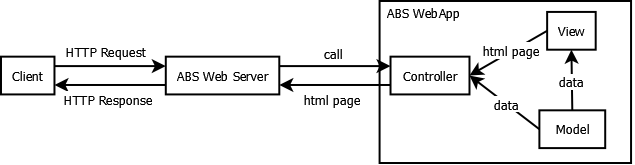
\includegraphics[width=0.8\textwidth]
        {img/abs-mvc.png}
    \caption{Skema framework ABS}
\end{figure}

\begin{figure}
    \centering
    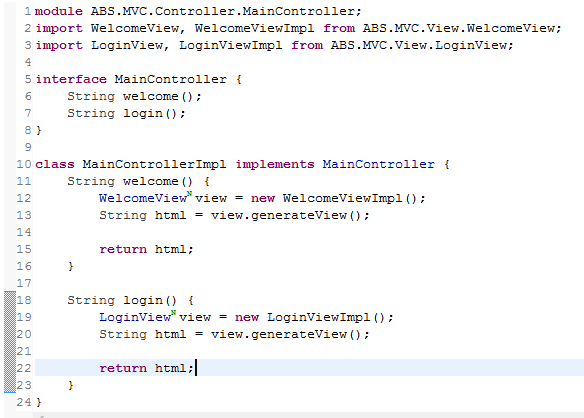
\includegraphics[width=0.8\textwidth]
        {img/controller-eksperimen.png}
    \caption{Contoh Controller}
\end{figure}

\begin{figure}
    \centering
    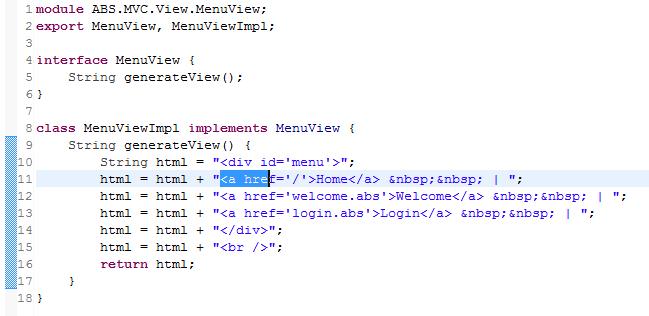
\includegraphics[width=0.8\textwidth]
        {img/view-eksperimen.png}
    \caption{Contoh ABS View}
\end{figure}

\begin{figure}
    \centering
    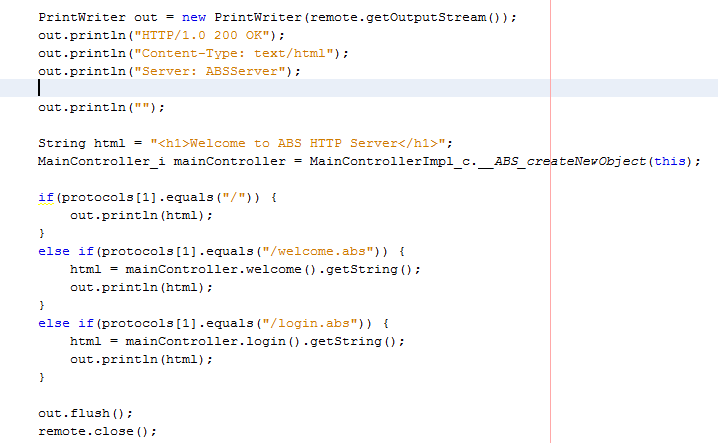
\includegraphics[width=0.8\textwidth]
        {img/server-eksperimen.png}
    \caption{Contoh ABS Server yang dibuat}
\end{figure}

\begin{figure}
    \centering
    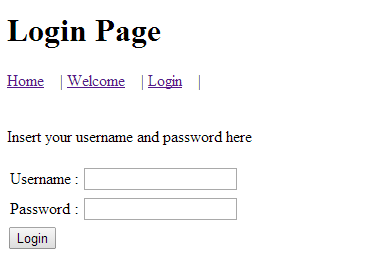
\includegraphics[width=0.8\textwidth]
        {img/login-page.png}
    \caption{Contoh halaman HTML yang dihasilkan dari ABS}
\end{figure}

%---------------------------------------------------------
\section{Rumusan Masalah}
%---------------------------------------------------------
\noindent
Berikut ini adalah rumusan masalah yang diperoleh dari hasil studi literatur dan percobaan awalan yang telah dilakukan oleh penulis sampai saat ini:

\begin{enumerate}
    \item Bagaimana strategi yang tepat dalam melakukan pemetaan bahasa pemodelan ABS ke dalam pola Model, View dan Controller dengan tetap mempertahankan kaidah-kaidah yang ada sesuai dengan studi literatur yang telah dilakukan.
    \item Arsitektur perangkat lunak seperti apakah yang cocok untuk pengembangan SPL berbasis dengan menggunakan bahasa pemodelan ABS.
    \item Bagaimana strategi implementasi yang dapat dilakukan agar \textit{framework} ABS yang dibuat dapat mendukung fitur \textit{delta modelling} yang dimiliki oleh ABS. 
\end{enumerate}

%---------------------------------------------------------
\section{Ruang Lingkup Penelitian}
%---------------------------------------------------------
\noindent
Adapun ruang lingkup dari penelitian ini adalah tentang perancangan dan perumusan strategi pengembangan \textit{framework} MVC SPL berbasis web dengan menggunakan bahasa pemodelan ABS. Harapannya, melalui penelitian ini penulis dapat menghasilkan sebuah \textit{framework} ABS yang dapat digunakan untuk melakukan pengembangan SPL berbasis web dengan menggunakan bahasa pemodelan ABS. Berdasarkan ruang lingkup tersebut, maka poin-poin pengerjaan yang akan dilakukan oleh penulis dalam penelitian ini antara lain adalah:

\begin{enumerate}
    \item Melakukan analisa terhadap sintaks dan aturan-aturan yang berlaku pada bahasa pemodelan ABS untuk kemudian dapat dirumuskan strategi dalam melakukan pemetaan bahasa pemodelan ABS kedalam komponen-komponen \textit{Model, View} dan \textit{Controller}.
    \item Merancang arsitektur dan strategi pengembangan \textit{framewok} ABS agar dapat mendukung fitur \textit{delta modelling} yang dimiliki oleh ABS.
    \item Membuat framework ABS berdasarkan strategi dan rancangan yang telah dilakukan sebelumnya.
\end{enumerate}

%---------------------------------------------------------
\section{Batasan Penelitian}
%---------------------------------------------------------

Dikarenakan adanya keterbatasan dalam hal pengetahuan, waktu pengerjaan dan fokus pengerjaan maka penulis menentukan batasan-batasan penelitian untuk penelitian kali ini yang diantaranya adalah:

\begin{enumerate}
    \item \textit{Framework} yang dibuat belum mendukung akses database karena untuk masalah akses \textit{database} pada ABS sudah menjadi topik penelitian tersendiri.
    \item \textit{Web Server} yang dibuat hanya berupa \textit{web server} sederhana dengan fungsionalitas terbatas pada menerima \textit{HTTP Request}, meneruskan \textit{request} tersebut ke ABS, serta mengirimkan \textit{HTTP Response} yang diberikan oleh ABS ke web browser. Oleh karena itu, penulis tidak akan mempertimbangkan masalah keamanan data, efisiensi dari \textit{web server} ataupun masalah \textit{concurency access} pada \textit{web server}.
    \item Penulis tidak melakukan komparasi antara \textit{framework} MVC yang dibuat dengan \textit{framework} MVC sejenis dikarenakan masih minimnya literatur yang membahas tentang pengembangan \textit{framework} MVC SPL berbasis web untuk bahasa pemodelan ABS.
\end{enumerate}

%---------------------------------------------------------
\section{Potensi Hambatan}
%---------------------------------------------------------

Adapun potensi hambatan yang diperkirakan akan muncul selama menjalani proses penelitian ini antara lain adalah:

\begin{enumerate}
    \item Sulitnya mendapatkan narasumber yang dapat ditanyakan tentang detail dari bahasa pemodelan ABS itu sendiri. Hal ini terjadi dikarenakan para ahli yang mengerti secara detail tentang bahasa pemodelan ABS semuanya berada di Eropa.
    \item Minimnya literatur tentang pemanfaatan bahasa pemodelan ABS untuk pengembangan SPL berbasis web.
\end{enumerate}